\section{Appendix}
\subsection{Full sized images vs. halved sized images}
In another experiment it was investigated whether the model performances would change if the full sized images were used rather than the half sized images. In \autoref{fullsize} four modified U-Net models initialized with the ImageNet weights were trained first on a dataset where the images were halved and then where the images kept their full size. On both datasets using the full sized images seems to make the models converge considerably faster. For the models trained on the original dataset the validation loss seems to be lower when the images are halved while the training loss seems to be about the same. However, when using data from the original, large rotation, horizontal and vertical datasets the validation loss seem to be higher for the halved images, but the training loss seems be lower.
\begin{figure}[H]
	\centering
	\begin{subfigure}[b]{0.24\linewidth}
		\centering
		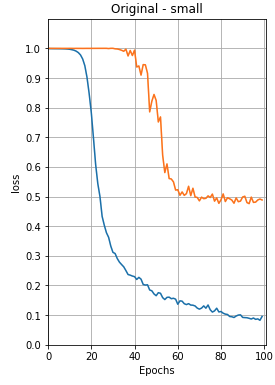
\includegraphics[width=\linewidth]{Materials/Results/Augmentation/Original}
		\caption{Model trained on original dataset with halved sizes.\newline\newline}
	\end{subfigure}
	\hfill
	\begin{subfigure}[b]{0.24\linewidth}
		\centering
		\includegraphics[width=\linewidth]{Materials/Results/Fullsize/originalfull}
		\caption{Model trained on original dataset with full sizes.\newline\newline}
	\end{subfigure}
	\hfill
	\begin{subfigure}[b]{0.24\linewidth}
		\centering
		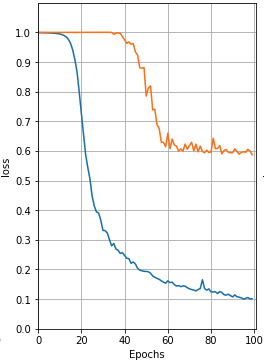
\includegraphics[width=\linewidth]{Materials/Results/Fullsize/augsmall}
		\caption{Model trained on original, large rotations, horizontal and vertical dataset with halved sizes.}
	\end{subfigure}
	\hfill
	\begin{subfigure}[b]{0.24\linewidth}
		\centering
		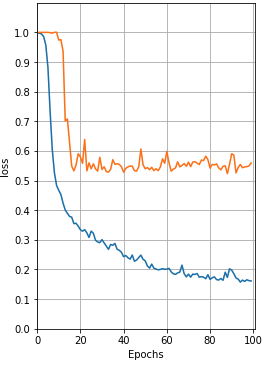
\includegraphics[width=\linewidth]{Materials/Results/Fullsize/augfull}
		\caption{Model trained on original, large rotations, horizontal and vertical dataset with full sizes.}
	\end{subfigure}
	\caption{Experiment showing the effect of training on full sized images vs. halved sized images.}
	\label{fullsize}
\end{figure}

\subsection{Test results}
\begin{figure}[H]
	\centering
	\begin{subfigure}[b]{\linewidth}
		\centering
		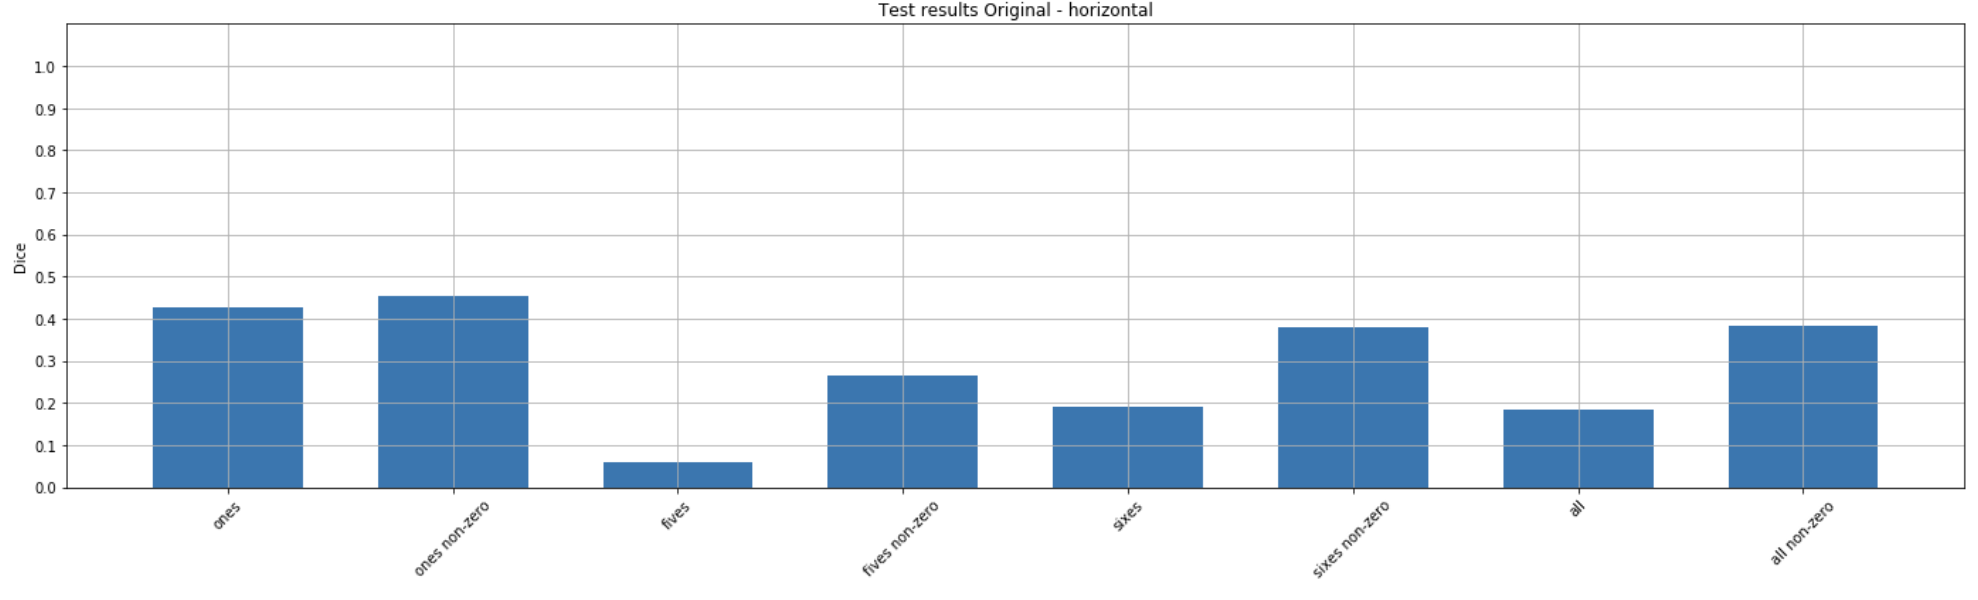
\includegraphics[width=\linewidth]{Materials/Appendix/OH}
		\caption{Results for the model trained on the original and horizontal data sets.}
	\end{subfigure}
	\caption{Average DICE on test set split into three separate volumes consisting of the single series images, five series images and six series images.}
\end{figure}
\begin{figure}[H]
	\centering
	\begin{subfigure}[b]{\linewidth}
		\centering
		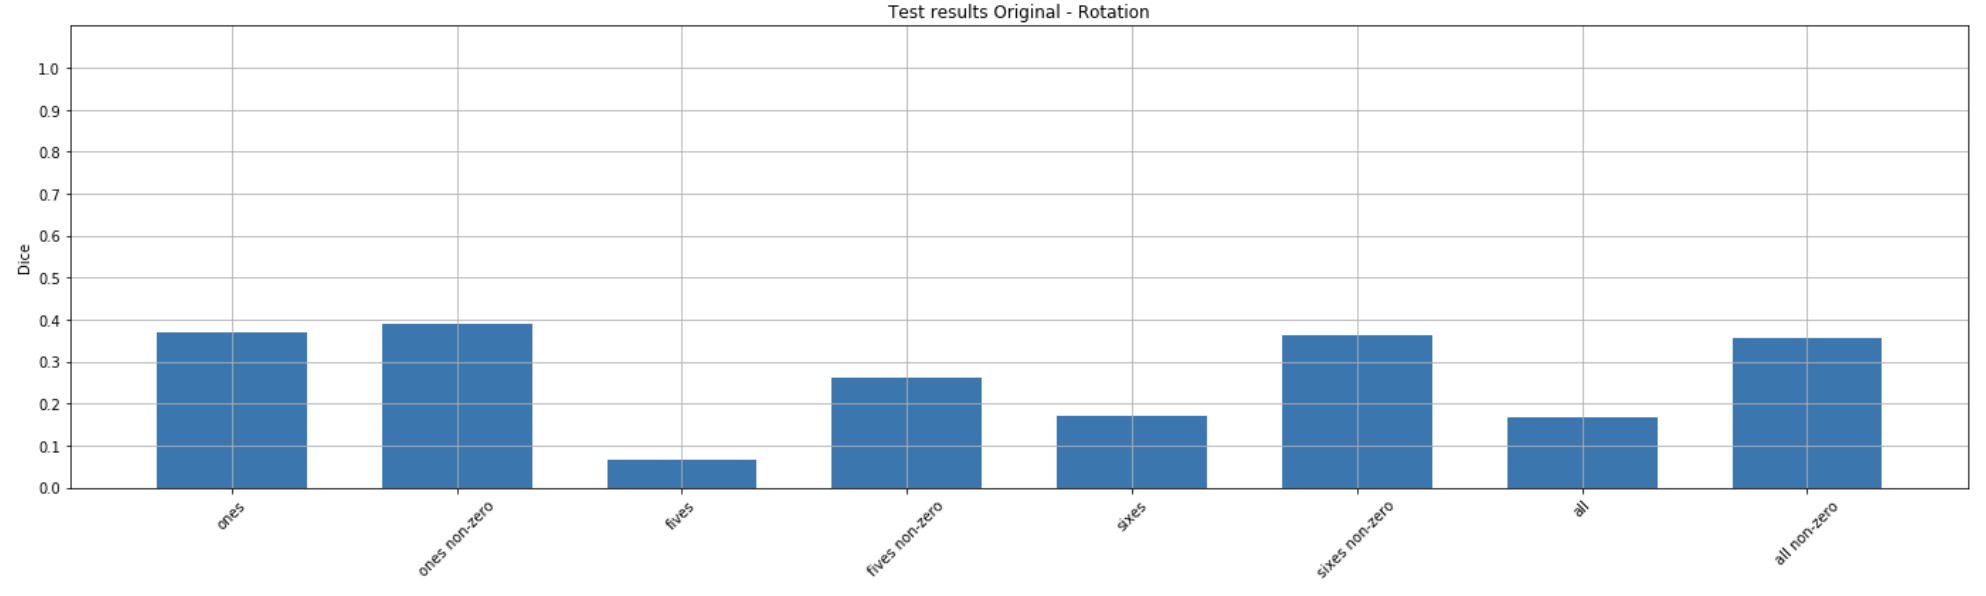
\includegraphics[width=\linewidth]{Materials/Appendix/OR}
		\caption{Results for the model trained on the original and large rotations data sets.}
	\end{subfigure}
	\\
	\begin{subfigure}[b]{\linewidth}
		\centering
		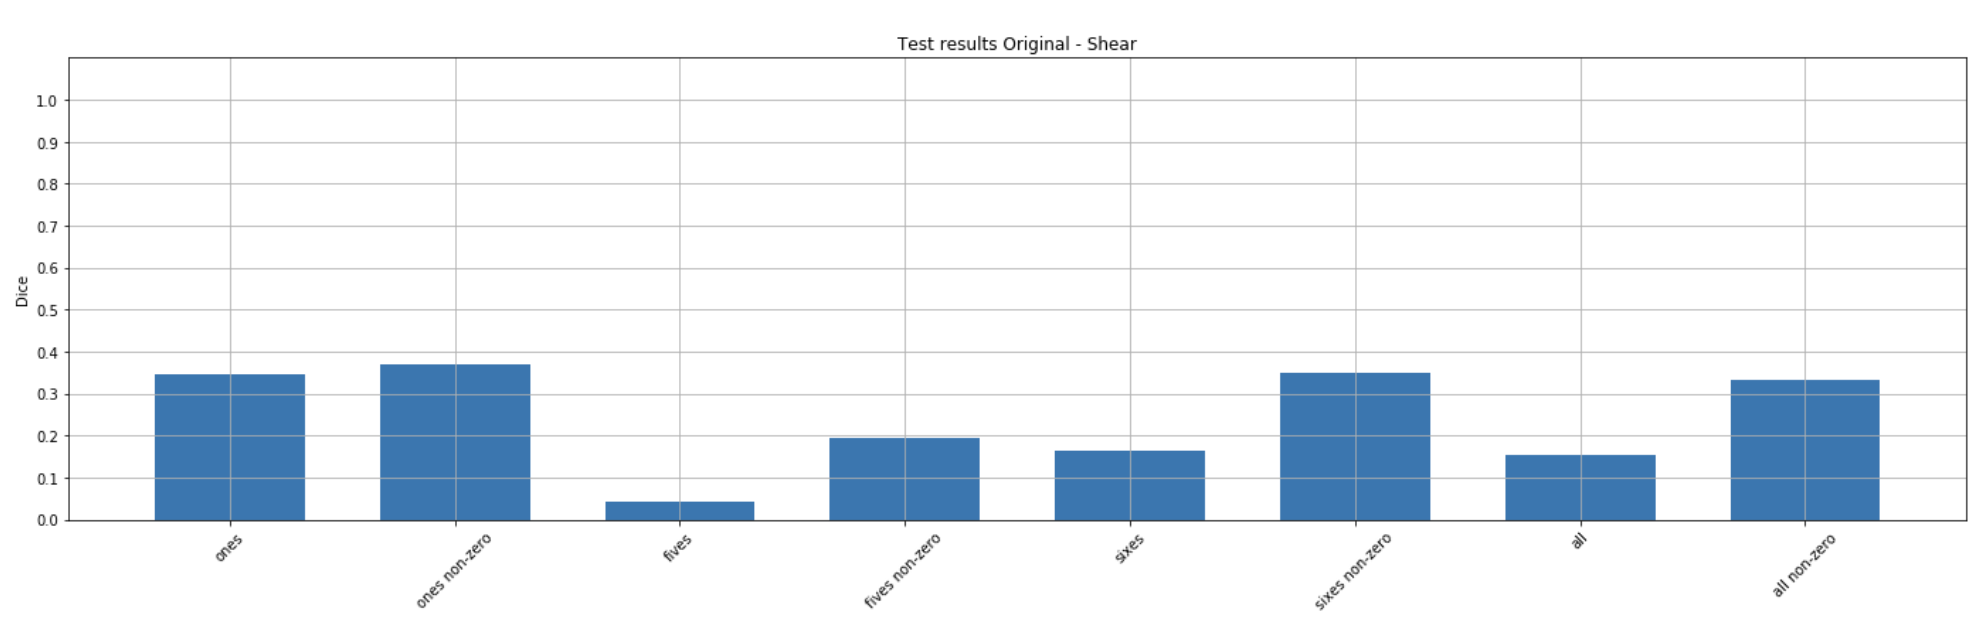
\includegraphics[width=\linewidth]{Materials/Appendix/OS}
		\caption{Results for the model trained on the original and large shearing data sets.}
	\end{subfigure}
	\\
	\begin{subfigure}[b]{\linewidth}
		\centering
		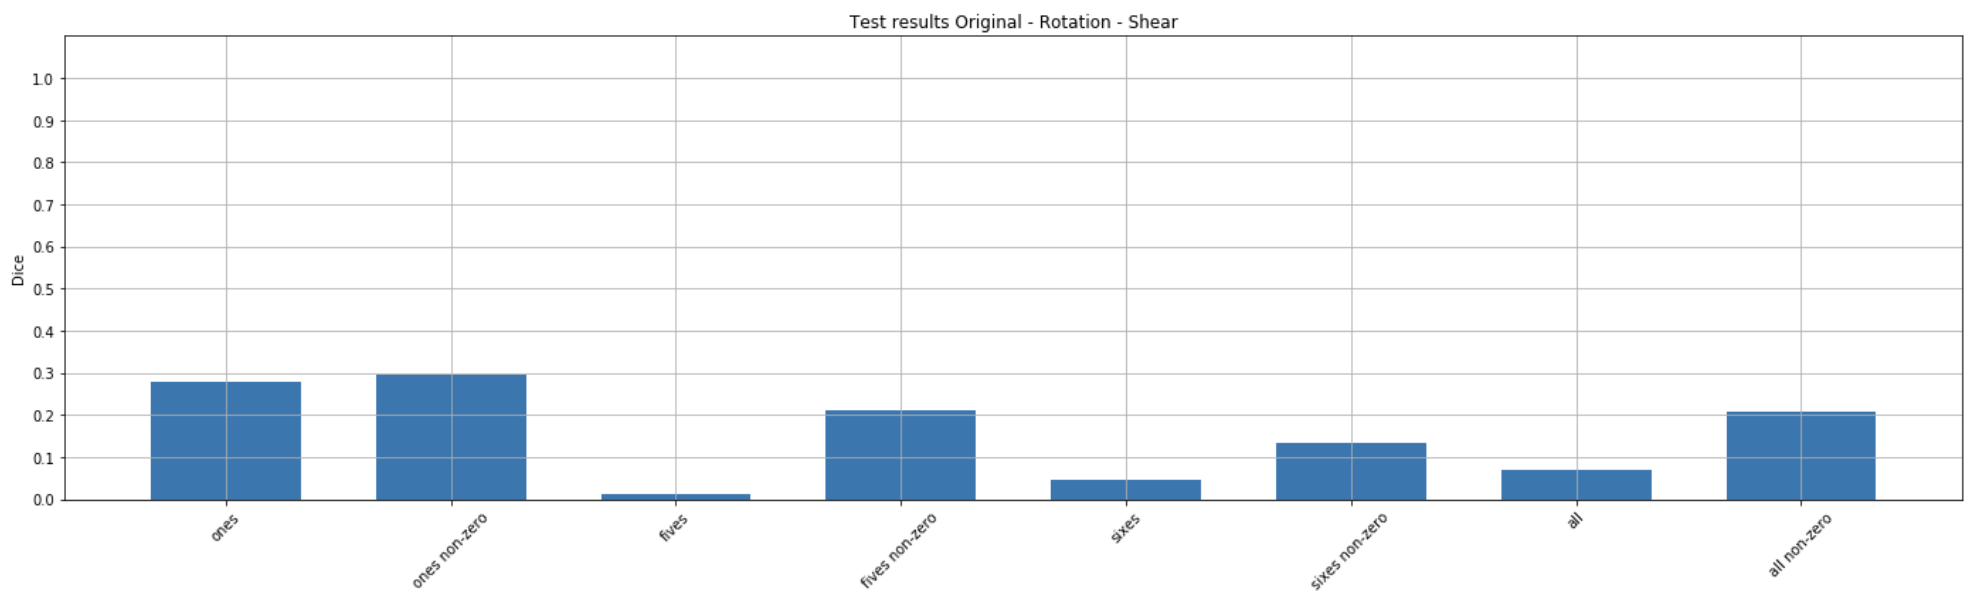
\includegraphics[width=\linewidth]{Materials/Appendix/ORS}
		\caption{Results for the model trained on the original, large rotations and large shearing data sets.}
	\end{subfigure}
	\\
	\begin{subfigure}[b]{\linewidth}
		\centering
		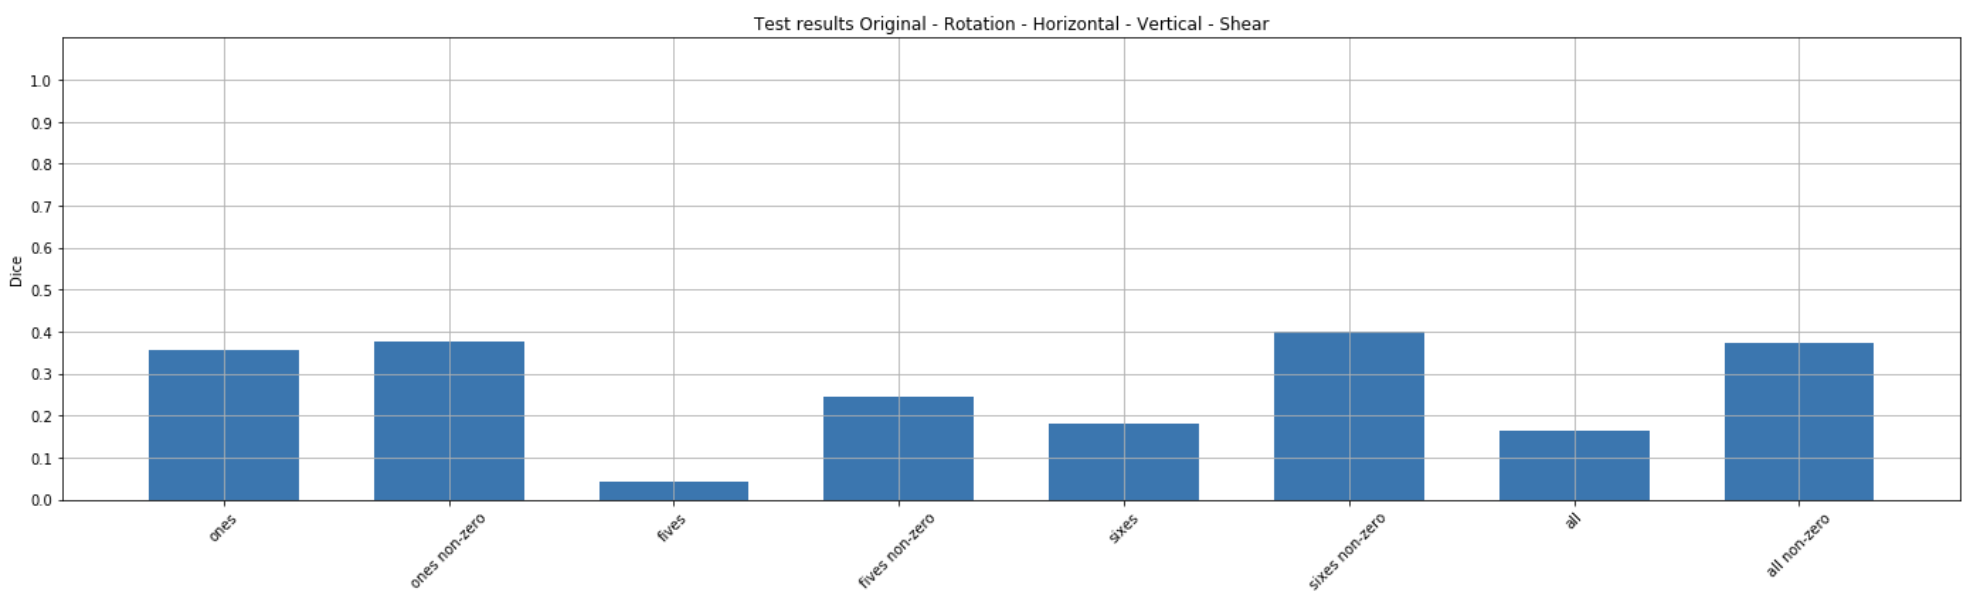
\includegraphics[width=\linewidth]{Materials/Appendix/ORHV}
		\caption{Results for the model trained on the original, large rotations, horizontal and vertical data sets.}
	\end{subfigure}
	\caption{Average DICE on test set split into three separate volumes consisting of the single series images, five series images and six series images.}
\end{figure}
\begin{figure}[H]
	\centering
	\begin{subfigure}[b]{\linewidth}
		\centering
		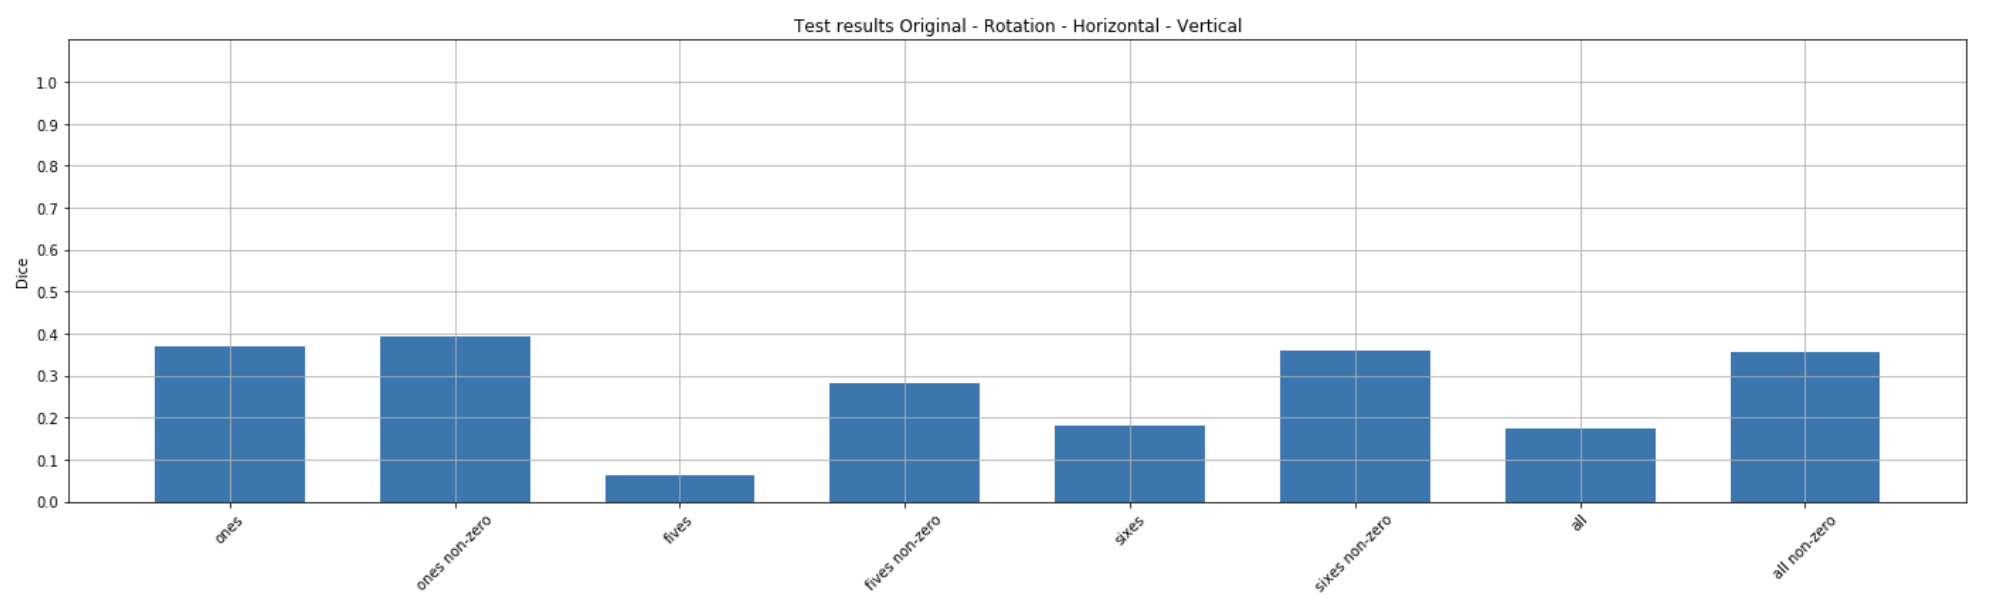
\includegraphics[width=\linewidth]{Materials/Appendix/ORHVS}
		\caption{Results for the model trained on the original, large rotations, horizontal, vertical and large shearing data sets.}
	\end{subfigure}
	\caption{Average DICE on test set split into three separate volumes consisting of the single series images, five series images and six series images.}
\end{figure}

\subsection{Prediction examples}
Here we see predicted masks versus the corresponding true mask for different models and images in the training set.

\begin{figure}[H]
	\centering
	\begin{subfigure}[b]{0.23\linewidth}
		\centering
		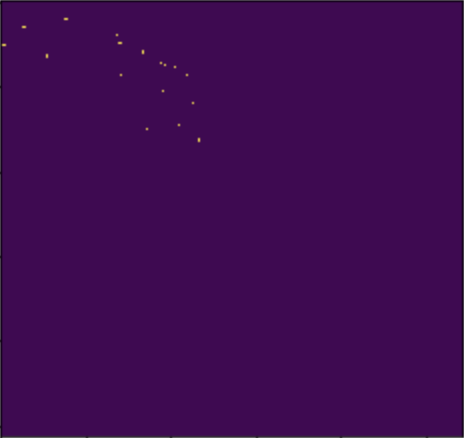
\includegraphics[width=\linewidth]{Materials/Appendix/results/O30R30SPred}
		\caption{Predicted mask from model trained on original, small rotations and small shearing. 0.93 DICE.}
	\end{subfigure}
	\hfill
	\begin{subfigure}[b]{0.23\linewidth}
		\centering
		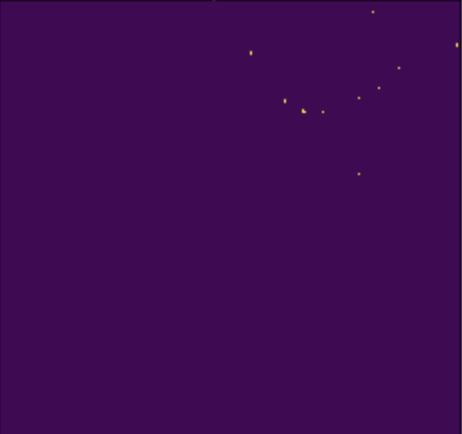
\includegraphics[width=\linewidth]{Materials/Appendix/results/imgaugPred}
		\caption{Predicted mask from imgaug model. 0.87 DICE.\newline\newline}
	\end{subfigure}
	\hfill
	\begin{subfigure}[b]{0.23\linewidth}
		\centering
		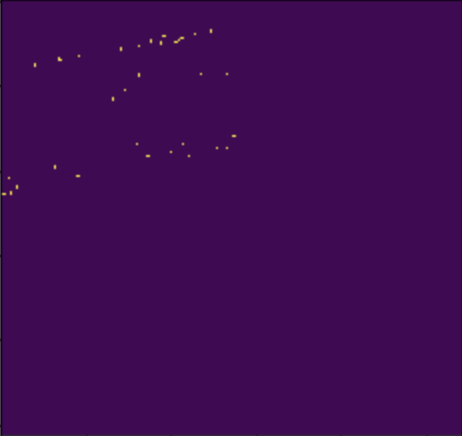
\includegraphics[width=\linewidth]{Materials/Appendix/results/originalPred}
		\caption{Predicted mask from model trained on original training set. 0.93 DICE.\newline}
	\end{subfigure}
	\hfill
	\begin{subfigure}[b]{0.23\linewidth}
		\centering
		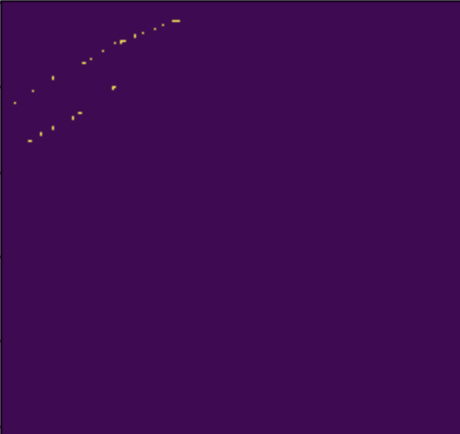
\includegraphics[width=\linewidth]{Materials/Appendix/results/OHPred}
		\caption{Predicted mask from model trained on original and horizontal data sets. 0.90 DICE.}
	\end{subfigure}
	\\
	\begin{subfigure}[b]{0.23\linewidth}
		\centering
		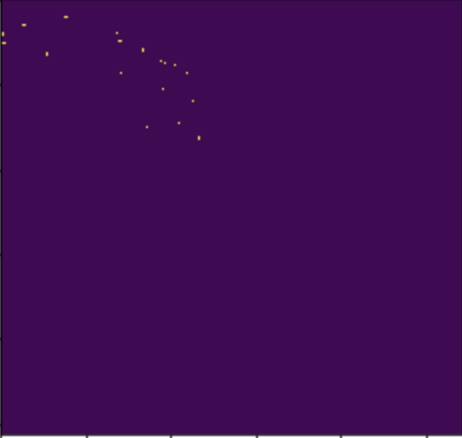
\includegraphics[width=\linewidth]{Materials/Appendix/results/O30R30SMask}
		\caption{True mask from model trained on original, small rotations and small shearing.}
	\end{subfigure}
	\hfill
	\begin{subfigure}[b]{0.23\linewidth}
		\centering
		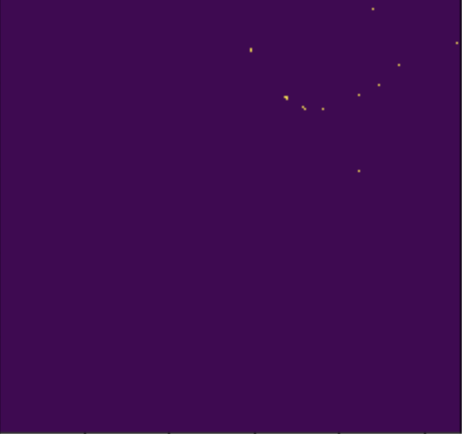
\includegraphics[width=\linewidth]{Materials/Appendix/results/imgaugMask}
		\caption{True mask from imgaug model.\newline\newline}
	\end{subfigure}	
	\hfill
	\begin{subfigure}[b]{0.23\linewidth}
		\centering
		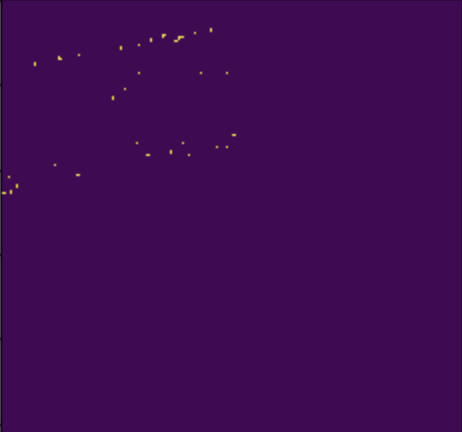
\includegraphics[width=\linewidth]{Materials/Appendix/results/originalMask}
		\caption{True mask from model trained on original training set.\newline}
	\end{subfigure}
	\hfill
	\begin{subfigure}[b]{0.23\linewidth}
		\centering
		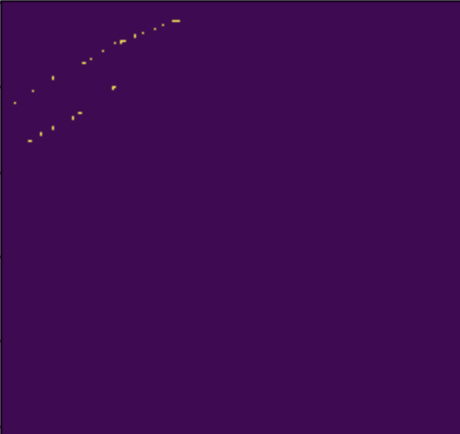
\includegraphics[width=\linewidth]{Materials/Appendix/results/OHPred}
		\caption{True mask from model trained on original and horizontal data sets.\newline}
	\end{subfigure}
\end{figure}